\customchapter{Product Overview}
% Add vertical space before the figure
\vspace{0pt} % Adjust the value (e.g., 10pt) to control the space
\section{Introduction}
The main aim of this project is to design a custom peripheral interfaced with the ARM microprocessor and deploy it on the Z-Board/Zybo FPGA. The peripheral is a 32 x 32 bit register having read and write access. A synthesised netlist of the custom SoC is deployed onto the FPGA and then further interfaced with the ARM core present on the zynq-7000 SoC (PS+PL) with the help of custom firmware. As a part of a test, one of the registers among the peripherals is used to send data to the LEDs present on the FPGA and another register is used to receive data from the switches on the FPGA. The design is scan-testable with the help of a TAP-controller and scan chain included to perform several test cases. The top-level system overview can be seen in the below figure.

% Add vertical space before the figure
\vspace{-15pt} % Adjust the value (e.g., 10pt) to control the space

\begin{figure}[h] % Use the 'h' option to try to place the image "here"
  \centering
  \setlength{\abovecaptionskip}{-10pt} % Reduce space above the caption
  \setlength{\belowcaptionskip}{-10pt} % Adjust space below the caption
  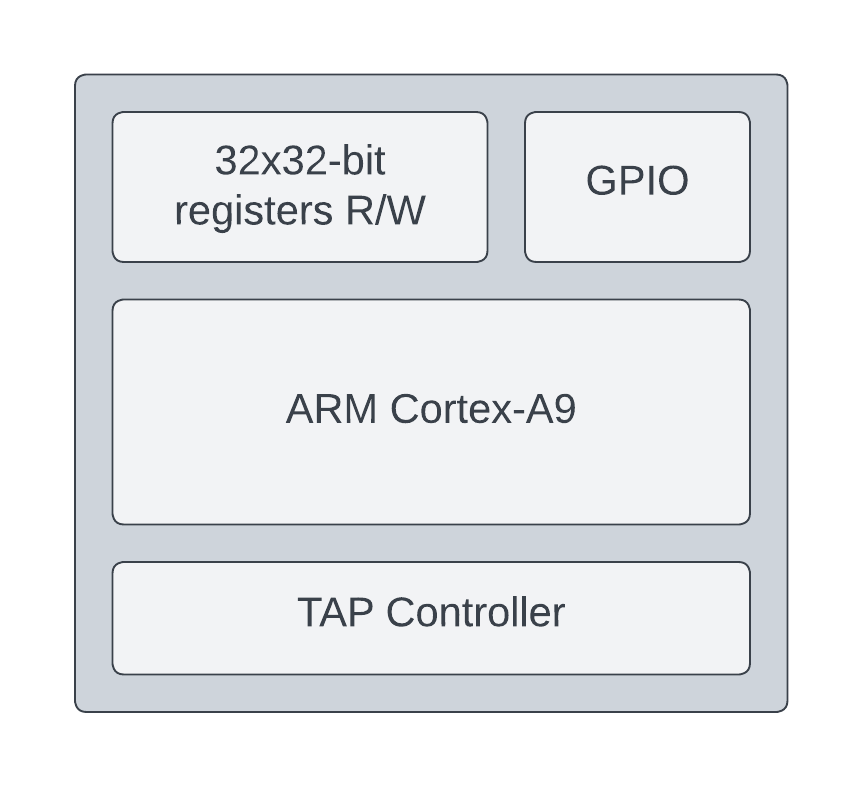
\includegraphics[width=0.5\textwidth]{Image/Block Diagram.png} % Replace 'your-image.png' with the actual file name
  \caption{System view}
  \label{Figure 1 : System view}
\end{figure}

\section{Key Features}
\begin{table}[H]
		%\begin{table}[ht]
		%\centering
  \begin{center}
		\begin{tabular}{|p{3cm}|p{5cm}|}
			\hline
			\textbf{Type} & \hspace{10mm}\textbf{Description} \\
			\hline \hline
			Processing Core &  ARM Cortex-A9   \\
            \hline
			Peripherals & 32x32-bit Registers \\
			\hline
			Bus System & AXI4-Lite \\
			\hline
			Debugger & Scan-Chain and TAP Controller \\
			\hline
		\end{tabular}
		\caption{\label{demo-table} Key Features}
		%\label{tab:01Glossary Type Descriptions}
  \end{center}
	\end{table}

\section{Functional Block Diagram}
The custom IP with 32x 32-bit registers is interfaced as a peripheral with the ARM Cortex-A9 core. The register file designed hereby acts as a slave and the ARM core acts as a master. Both master and slave are interfaced with the AXI4 lite bus. This bus ensures high-speed and reliable data communication between the register peripheral. The registers are RISC-V compliant hence they should be able to be used to execute any of the instructions from the RISC-V instruction set.  Hence, any firmware running on the Processing System (PS) of the SoC can use the registers on the Programmable Logic (PL) of the SoC as memory-mapped registers with the help of the AXI4 lite bus. Since this SoC will be deployed into the Zybo development board based on Zynq-7000 SoC, the LED’s and Switches present on the board can be accessed and interfaced with the help of custom register peripheral, ARM core and Custom firmware. In order to make the SoC scan testable, a TAP controller is implemented as per IEEE 1149.1 JTAG specification and interfaced with the register peripheral over a scan chain. This TAP controller receives instructions and test data from the JTAG network via standard JTAG serial pins.
\vspace{3mm}
% Add vertical space before the figure
\vspace{-15pt} % Adjust the value (e.g., 10pt) to control the space

\begin{figure}[h] % Use the 'h' option to try to place the image "here"
  \centering
  \setlength{\abovecaptionskip}{-10pt} % Reduce space above the caption
  \setlength{\belowcaptionskip}{-10pt} % Adjust space below the caption
  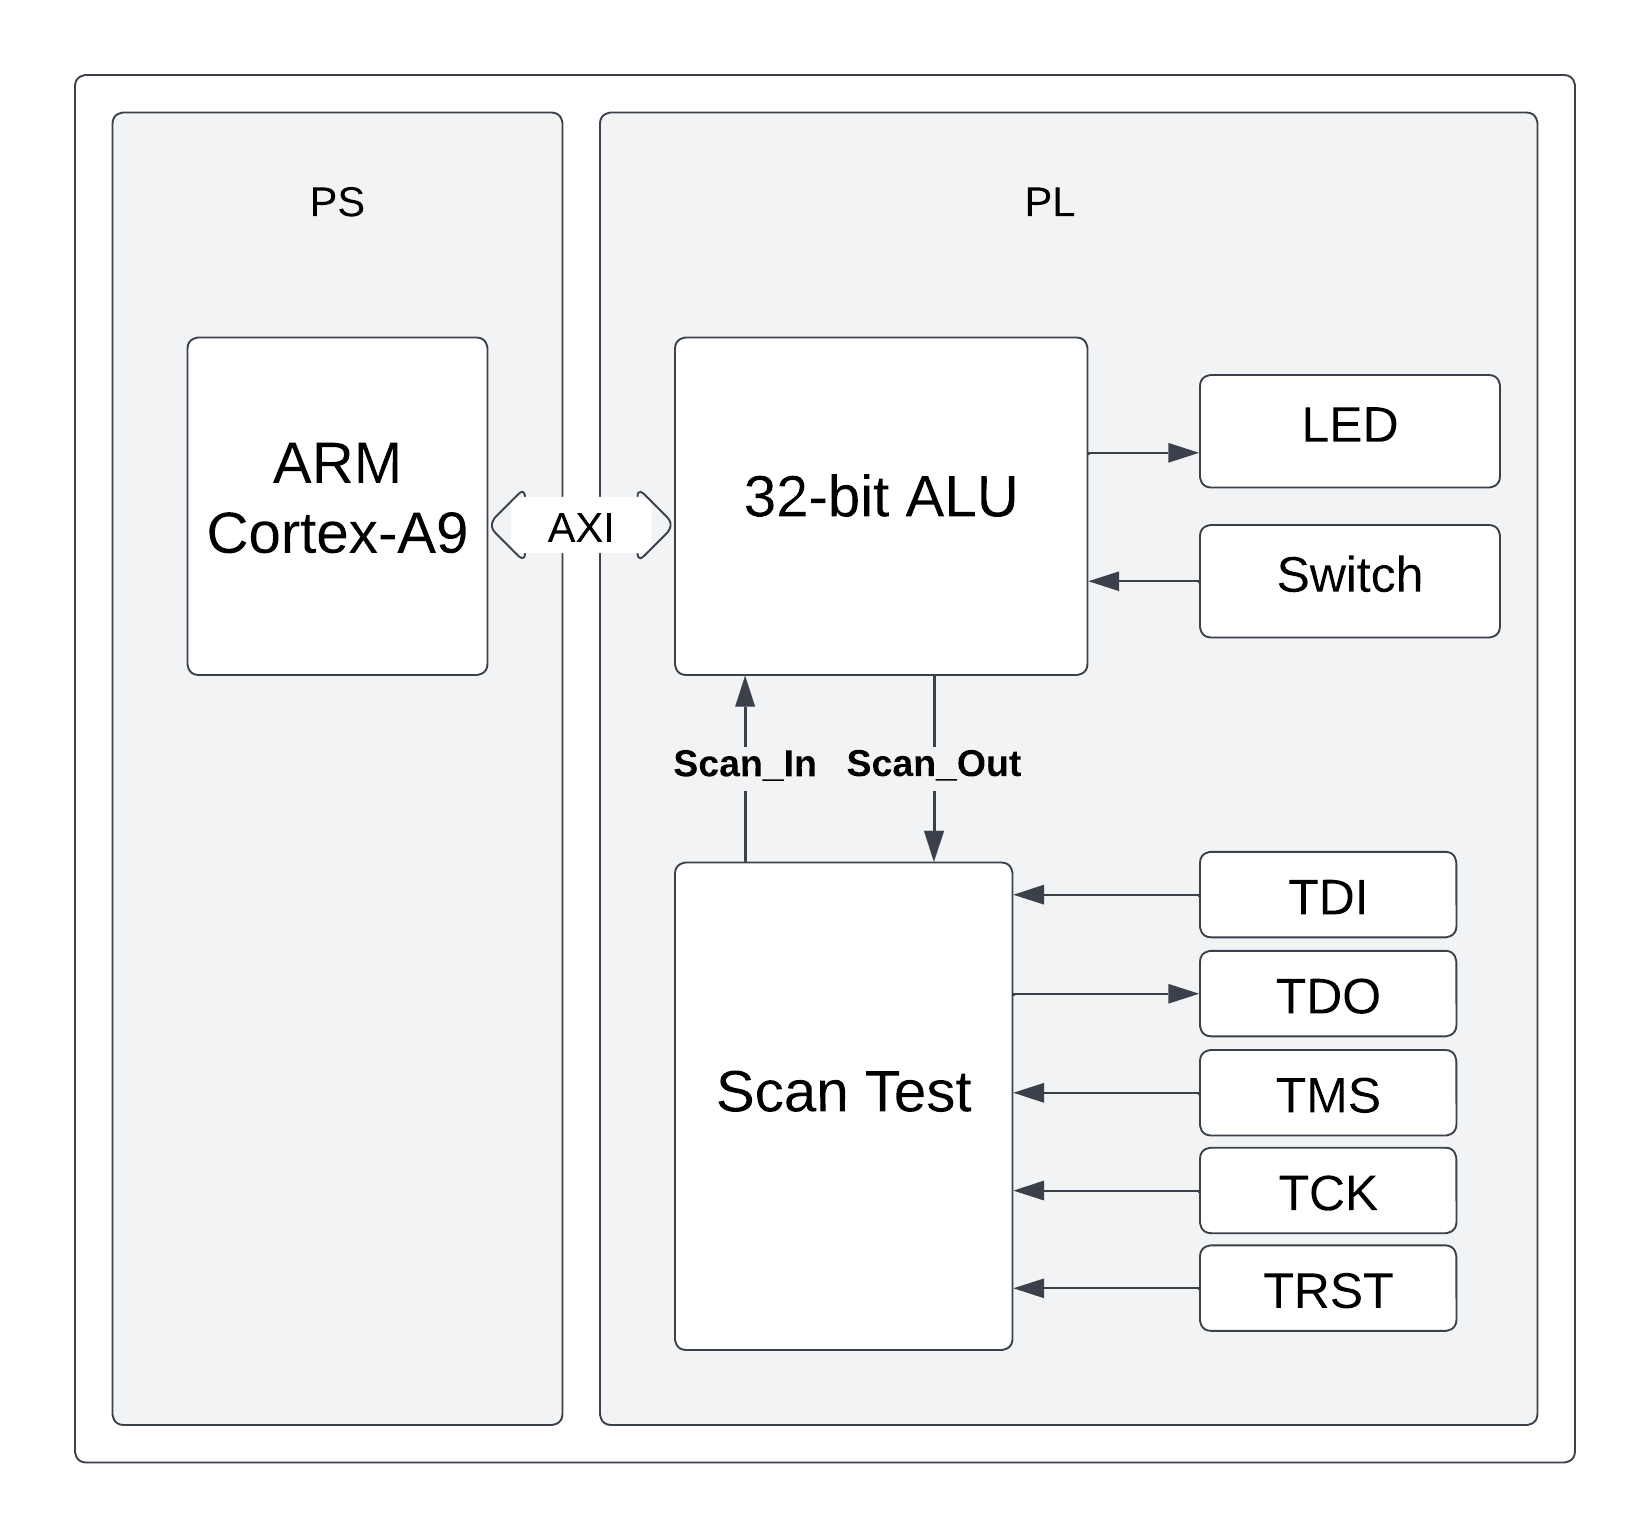
\includegraphics[width=0.7\textwidth]{Image/ARM.png} % Replace 'your-image.png' with the actual file name
  \caption{Functional Block Diagram}
  \label{Figure 1 : Functional Block Diagram}
\end{figure}

% register file reshuffle

% Start a new page after the figure



